\section{How to build a \gls{name}}

In the current incarnation of \glspl{name}, we intervene during programmers' web browser.
Each \gls{name} or explainer for a language or library is implemented on a web server.
When queried with the text of a web page, the \gls{name} detects instances of the language, parses them, and returns explanations for each one as formatted HTML that can be viewed in a tooltip.
These steps are decribed in detail below.

\begin{figure}
\centering{
    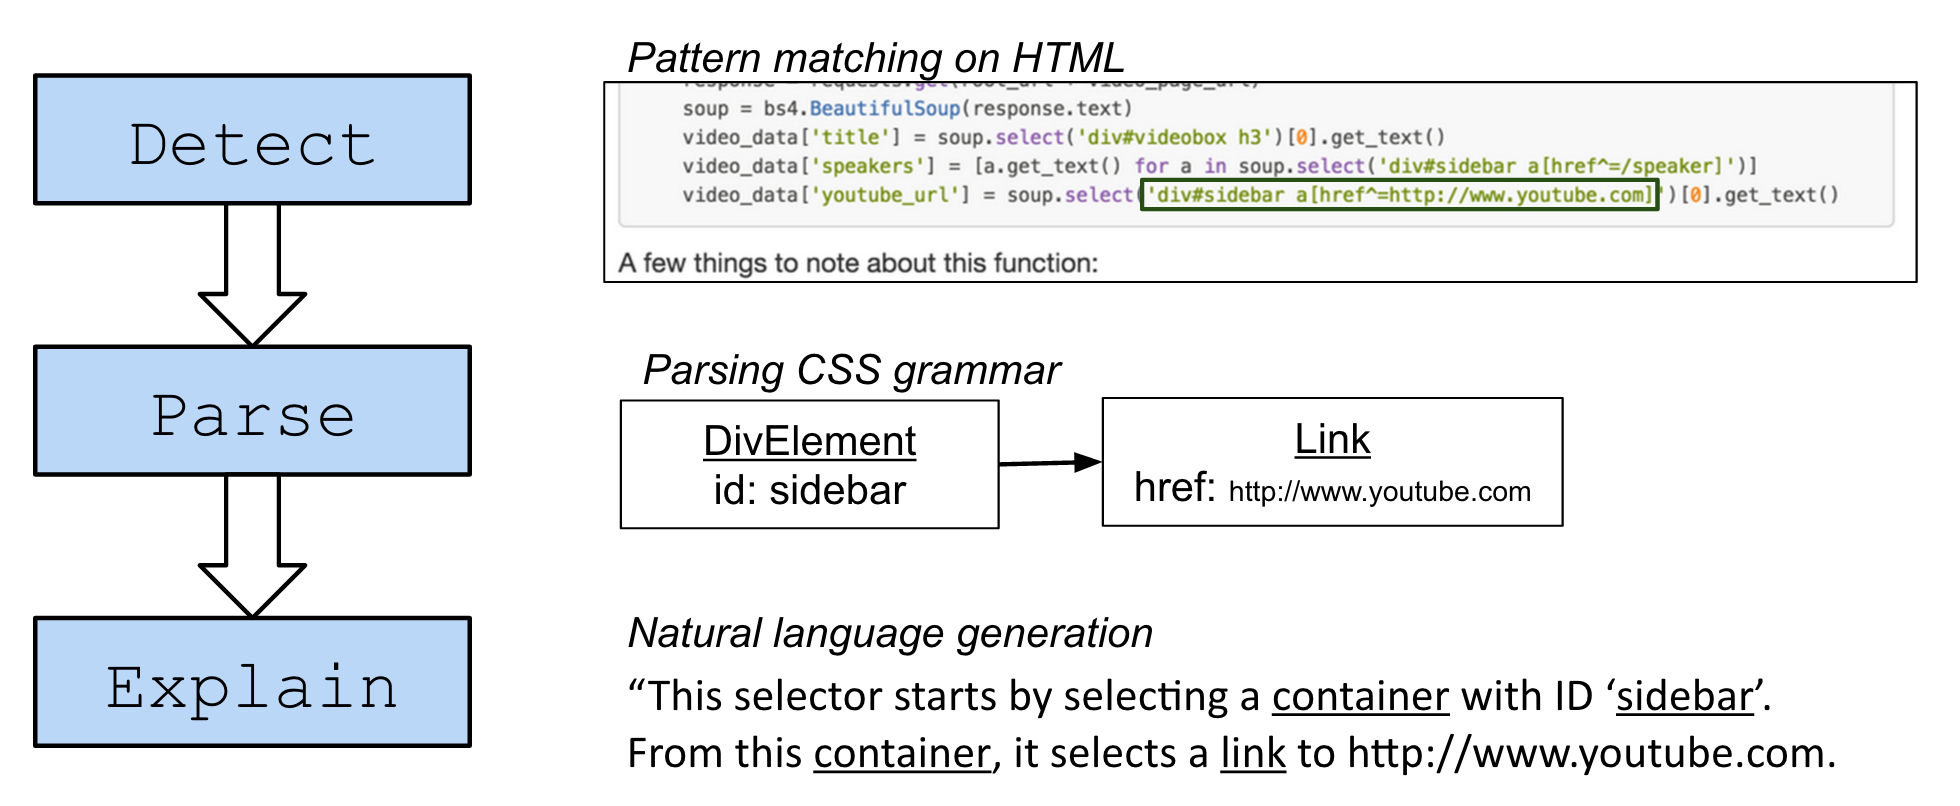
\includegraphics[width=.4\textwidth]{figures/explanation_pipeline}
}
\caption{\Glspl{name} \emph{detect} relevant code snippets, \emph{parse} them, and then \emph{generate explanations}.  Here we show examples of the output of each stage of the pipeline for a \gls{name} that explains CSS selectors.}
\label{fig:explanation_pipeline}
\end{figure}

Programmers access explanation servers by triggering a \emph{bookmarklet} for the server, a short web script that can be embedded in the bookmarks bar (Figure~\ref{fig:click_bookmarklet}).
This bookmarklet queries the server with the page source, and receives an explanation of all instances of the language.
From then on, any time they select text for which an explanation has been generated, it will appear in a tooltip overlaid on the document, directly beneath the source (Figure~\ref{fig:explain_on_select}).

\begin{figure}
\centering{
    \subfigure[A user enables explanations by clicking on the bookmarklet to activate descriptions for the language or library.]{
        \framebox{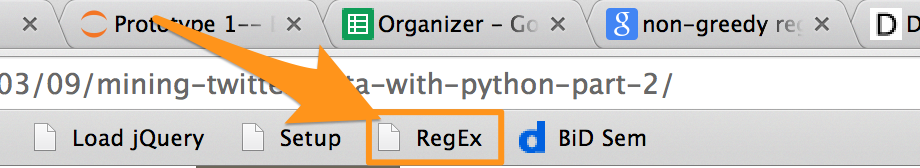
\includegraphics[width=.4\textwidth]{figures/click_bookmarklet}}
        \label{fig:click_bookmarklet}
    }
    \subfigure[Once explanations are activated, users can view explanations for relevant snippets by just selecting their text.\andrew{Replace with non-third party explanation.}]{
        \framebox{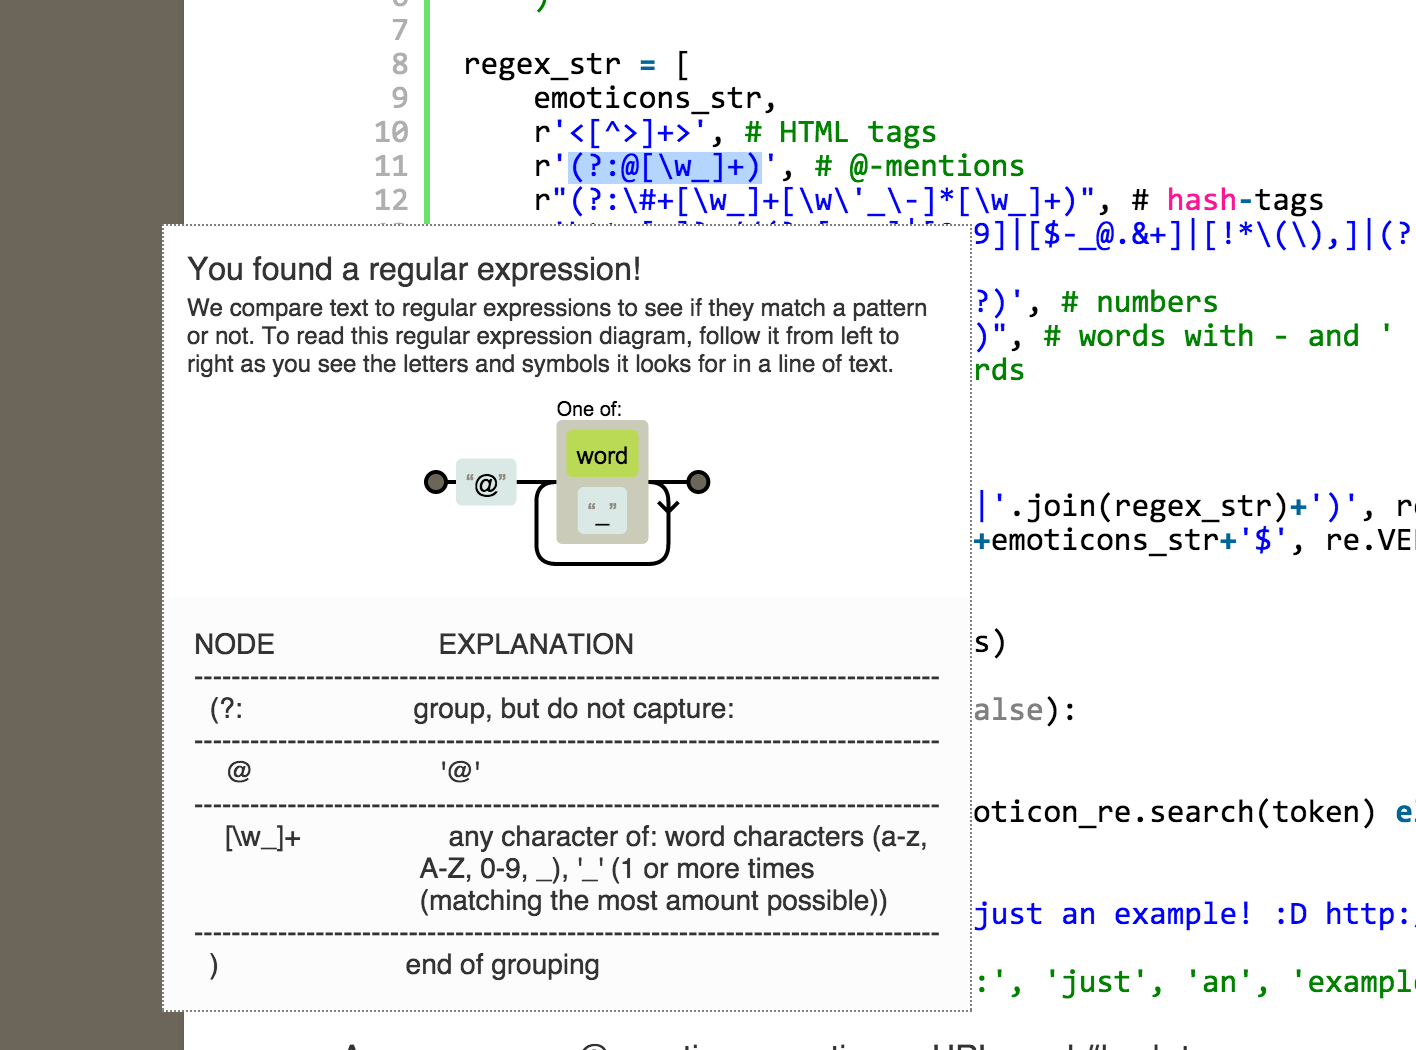
\includegraphics[width=.4\textwidth]{figures/explain_on_select}}
        \label{fig:explain_on_select}
    }
}
\end{figure}

In a world where \glspl{name} were prevalent and many existed for each language and library, how would we make sure multiple \glspl{name} didn't try to explain the same code?
We expect that in future versions, users can manage languages and libraries they want to explain from a central configuration interface.
Toolbars can be added to the browser to allow users to rapidly turn off explanations that they don't need.

Detecting explainable code.

Parsing code snippets.

Generating explanations and HTML.

Limitations on the types of code we can read and process.
